\documentclass[letterpaper,9pt]{article}
\usepackage{extsizes}
\usepackage{fullpage}
\usepackage{amsmath,amsfonts,amssymb}
\usepackage{cite}
\usepackage{hyperref}
\usepackage{graphicx}
\title{Assignment 1: Problem 1}
\author{Ernesto Rodriguez}

\newcommand{\vectornorm}[1]{\left|\left|#1\right|\right|}
\DeclareMathOperator*{\argmin}{\arg\!\min}

\newcommand{\networkSpecs}[6]{
  \begin{center}
  \begin{tabular}{ | l | c | }
    \hline
    \multicolumn{2}{|c|}{{\bf Network Specifications}} \\
    \hline
    {\bf Bias Vector} ${\bf x}^{bias}$ & $\mathcal{N}(#1)$ \\
    \hline
    {\bf Spectral Radius} $|\sigma_i|_{max}$ & #2 \\
    \hline
    {\bf Output Feedback Weights} ${\bf W}^{back}$ & $\mathcal{U}(#3)$ \\
    \hline
    {\bf Leaking Rate} $\lambda$ & #4 \\
    \hline
    {\bf Regularization} $\alpha$ & #5\\
    \hline
    {\bf MSE} & #6\\
    \hline
  \end{tabular}    
  \end{center}
}

\begin{document}

\Huge{\bf Training Echo State Networks with Short Segments of Motion Capture Data\\[1cm]}
\large{\bf Ernesto Rodriguez\\[0.5cm]}
\emph{Computer Science \\ Jacobs University Bremen \\ College Ring 7 \\ 28759 \\ Bremen \\ Germany\\[0.5cm]}
\emph{Type: Guided Research Proposal \\ Date: December 9th, 2012 \\ Supervisor: Prof. Dr. Herbert J\"{a}ger\\}
\line(1,0){520}\\ \\
\Large{\bf Abstract\\ \\}

Motion capture data is used in the gaming and film industry for a variety of purposes. This data is obtained by attaching markers to a human and recording his movements which is a task that requires time and equipment. There are applications that can benefit from long streams of periodic data. The freely available streams are usually short lasting only a couple of steps. They can be extended by repeating the motion several times but that might be too homogeneous. This paper proposes the usage of Echo State Networks (ESNs) to learn motion patterns and repeat them in a way that evolves as a non-linear dynamical system. Echo State Networks are a machine learning tool for working with discrete and continuous time series. They have archived good results in a variety of tasks without requiring many parameters to be adjusted. This paper shows how Echo State Networks can be used to learn periodic human movements encoded as motion capture data. The main challenge is dealing with short data sets since the motion must be learned from very few samples. There are many important parameters that should be adjusted in order to archive good quality and this paper explains how theese parameters were tuned. \\

\noindent\line(1,0){520}

\pagebreak

\tableofcontents

\pagebreak

\section{Introduction}

The human being is capable of performing many diverse types of movements. A subset of these movements involve periodic motions which can be seen as a periodic signal evolving over time. This signal although it looks regular when viewed from the broad perspective, it has small irregularities all over its repetitions. The system should be able to generalize the regular patterns and discard the irrelevant irregularities to reproduce human movement.\\

This research addresses the challenge of learning human movements using small training data sets. This creates the challenge of learning how many degrees of freedom, consisting of the rotations from many of the human bones, influence each other with very few samples. The inspiration behind this goal is figuring out whether human motion can be quickly learned by a computer since common intuition suggests that movements should be learnable in an efficient manner because humans can usually learn a movement after very few (even one) repetition. This paper doesn't intend to study learning from a biological perspective since the tools employed don't model biological structures.\\

The tool that will be used to learn these movements is Echo State Networks. Echo State Networks are a type of Recurrent Neural Networks which consist of connected nodes in such a way such that cyclic connections between nodes are permitted. Learning is usually done by optimizing the strength of the weights that connect the nodes in order to approximate a teacher signal as close as possible. As it was stated in \cite{JaegerESNTutorial}, Echo State Networks are a robust tool to learn continuous non-linear signals in a computationally efficient way \cite{Jaeger05TrainingRRN}. This indicates they might be suitable for learning human motions. \\

There have been previous attempts to teach human movements to computers. The most notable is \cite{GentHumanMotion} where Echo State Networks were used as the learning tool. In this paper the network successfully learned walking and running and could even generate smooth transitions between the movements without them being present in the training data. The success of this research is a good sign but in this case running and walking were used since there is a rich amount of training data for those motions and the networks used were much larger than the ones used in this work. This paper extends the work by investigating whether more motions can be learned with simpler networks and less training data. An approach based on energy and probability using a modified Restricted Boltzmann Machine is presented in \cite{TaylorModelingHuman}. This method was also successful to learn walking and running motion from a rich set of examples. It was also capable to generate transitions between motions and proved to be better than traditional methods to interpolate missing data in motion capture file. In contrast to ESNs which are a tool for general purpose  signal processing tasks, the method presented in \cite{TaylorModelingHuman} was specifically built to learn human motion (although the author argures it should work equally well for other tasks). Finally a biologically inspired approach is presented in \cite{Joshi05MovementGeneration} where spiking neurons are used to generate movements for a robotic arm after some training. The approach is significantly different since spiking neurons are a tool based on how the neurons of the human brain work. In this case the objective was to generate a signal to control an arm instead of learning and producing movements from motion capture data. Much simpler movements were produced in this case and the network had a more complicated structure and topology than Echo State Networks since it was built to resemble biological nervous structures. The network was capable of learning and producing control signals to move an arm. The simpler design of ESNs, the success from \cite{GentHumanMotion} and this work suggest that ESNs should also be effective for this task.\\

As it is discussed in \cite{ESNVerstraeten}, ESNs can used for a wide variety of applications by tuning very few parameters. Complimented with the fast training due to the efficiency of ESNs and the small size of the training set, it should be possible to quickly tune the parameters and produce reasonable results since the output of many different networks can be inspected and compared. ESNs have proven to be successful in various applications including learning human movements using rich training data sets. This research intends to explore wether ESNs can still be successful to learn human movements without a rich training data-set.


% Based on the success of ESNs in many tasks and in particular learning human movements from motion capture data this paper extends the previous work by investigating whether ESNs are still a reliable tool when only small training data-sets exists. Especially because ESNs require some training data to be used for initialization.

\subsection{Research Topic}

\subsection{Background}

Motion Capture Data encodes human movements using a skeleton and specifying the rotation on every possible degree of freedom for each of the bones. This leads to a signal which essentially boils down to a vector with many dimensions (up to 37 in this work) where the values of each entry are a function over time representing how the bone is positioned as the movement goes on. The data was obtained by placing markers on humans and tracking the position of their body parts while they were performing one of the movements. Since the movements were created in a `natural` way they contain actions that might be irrelevant since they result from the natural movement of humans which will never be repeated in the exact same way multiple times. It is also the case that some bones are more relevant than others in a particular movement but this depends on the movement being performed.\\

The signal mentioned above has many components that interact with each other, non-linearly, in a time dependent way. This results in a very complex signal which is repeated very few times. Even though learning a motion is something trivial for a human, the network must be capable of doing it without any context. For a computer, the signal carries no meaning other than the fact that future values of the signal can be predicted by observing the previous values. For this reason it is challenging to learn these interactions with very few samples. The computer must be capable of producing a model without any previous knowledge of what movement is. To overcome this challenge, many parameters of the neural network must be adjusted. Adjusting these parameters is the main challenge addressed in this research.\\

It is also worth noticing that so far there exists no underlying fundamental theory about Echo State Networks which would allow to optimally tune these parameters according to a specific data-set. This is an active field of research and guidelines exist which help archive better results by observing the behavior of various components of the network as it evolves. This research focuses on using these guidelines to allow Echo States Neural Networks to reproduce periodic human motions. The concepts introduced in this section will be formally specified in the following sections.

\subsection{General Objectives}

The general objective of this research is determining whether periodic human movements can be learned and reproduced by Echo State Networks using small training data-sets. This means data-sets that contain less than five repetitions of a particular motion. In terms of motion capture data, this usually means less than 400 time-steps.

\subsection{Specific Objectives}

To archive the main objective, the following sub-goals are set for the three motions treated in this paper:

\begin{itemize}
  \item Determine an appropriate value for the leaky integrator
  \item Determine an appropriate level of complexity of the model (the regularization parameter)
  \item Determine appropriate output feedback weights for the movement
  \item Generate a stable repetition of the learnt periodic movement
  \item Archive the objectives mentioned above with a network of 100 internal units.
  \item Provide guidelines to tune ESNs to learn motion capture data
\end{itemize}

\section{Background Topics}

During this research, various tools and methods were used. The following sections provide an introduction to these topics. Hopefully this should be enough information to understand the research but if additional knowledge is required the reader can consult the referenced material, in particular \cite{JaegerESNTutorial}.

\subsection{Echo State Neural Networks}

Neural networks are computational mechanisms originally inspired on the structure of the brain. Ever since they evolved to become a practical computational tool for signal processing. They consist of input nodes, internal or hidden nodes and output nodes. Depending on the way the nodes are connected to each other they are classified as recurrent neural networks or feed-forward neural networks. Echo state neural networks (ESNs) are a type of recurrent neural networks whose primary characteristic is that only connections from internal nodes to outputs are trained. Echo state neural networks are a powerful mechanism to reproduce time series as presented in \cite{JaegerESNTutorial}. The remainder of this section will be used to formally present echo state neural networks as they will be used in the research, which is based on \cite{JaegerESNTutorial,ESNVerstraeten}.\\

A time discrete network will be considered. The network has $N$ internal network nodes and $L$ output nodes. Note that networks without input nodes will be used in this research. The state of the network at a given time $t$ is ${\bf x}(t)=(x_1(t),x_2(t),..,x_N(t))$ and the output of the network at time $t$ is ${\bf y}(t)=(y_1(t),y_2(t),..,y_L(t))$. The connection weights between units are collected in matrices. A  $N \times N$ matrix ${\bf W}$ for the internal nodes, a $L \times N$ matrix ${\bf W^{out}}$ for connections between internal nodes and output nodes and a $N \times L$ matrix ${\bf W^{back}}$ output feedback matrix. A bias vector ${\bf x}^{bias}$ is sometimes used to destroy the sine symmetry of the network. This type of symmetry results from signals with periodic oscillations which result in network states where multiple state updates seem reasonable. A bias vector was also used \cite{GentHumanMotion} to model human movement. The state entries, weights, bias entries and outputs will all be real valued numbers.\\

The state of the network is updated according to the equation
\[
{\bf x}(t+1)= (\lambda {\bf x}(t)) + (1-\lambda){\bf f}({\bf Wx}(t) + {\bf W^{back}y}(t)) + {\bf x}^{bias}
\]
where,
\begin{itemize}
  \item ${\bf f}=(f_1,f_2,...,f_N)$ are the output functions of the internal units (usually sigmond functions).
  \item $\lambda$ is the leaking rate (see the following sections).
  \item ${\bf x}^{bias}$ is known as the bias vector.
\end{itemize}
The output of the network at time $t$ is given by the equation
\[
{\bf y}(t+1)={\bf f^{out}}({\bf W^{out}}{\bf x}(t))
\]
where,
\begin{itemize}
  \item ${\bf f^{out}}=(f_1^{out},f_2^{out},...,f_L^{out})$ is the output units functions
  \item $({\bf x}(t),{\bf y}(t))$ is the concatenation of the internal state and output vectors
\end{itemize}
The training procedure for ESNs goes as follows. Suppose we are given the output signal ${\bf y_{teach}}(t)$ for $t=0,..,t_{max}$. We wish to have a ESN whose output signal ${\bf y}(t)$ is as close as possible to ${\bf y_{teach}}(t)$. This is done as follows.\\\\
{\bf Produce a ESN} with $N$ input units and $L$ outputs where $L$ is the dimension of the vector ${\bf y}(t)$. Random sparse matrices are used to produce the ${\bf W}$ and ${\bf W^{out}}$. It is important that the network has echo states \cite{JaegerESNTutorial}. The usual recommendation is to scale the internal weights {\bf W} such that $|\sigma_i |_{max}$ close to $1$ where $\sigma_i$ are the eigenvalues of {\bf W}. The entries of the bias vector ${\bf x}^{bias}$ are obtained by sampling a normal distribution. Guidelines on how to produce such a network can be found in \cite{JaegerESNTutorial}.\\\\
{\bf Run the network} by teacher forcing the ${\bf y_{teach}}(t)$ signal into the network. Teacher forcing consists of replacing the network output ${\bf y}(t)$ with the value of ${\bf y_{teach}}(t)$. This means that the update function of the network is:
\[
{\bf x}(t+1)= (\lambda {\bf x(t)}) + (1-\lambda){\bf f}({\bf Wx}(t) + {\bf W^{back}y_{teach}}(t)) + {\bf x}^{bias}
\]
The network must be run in this way for some initial transient and the outputs during this transient will be discarded. It is better to discard a big amount of initial states, but the amount of data discarded also depends on the amount of training data available.\pagebreak

{\bf Collect the ESN output} for the remaining training data. We will denote with $t_{min}$ the time where the output began to be collected and $t_{max}$ the time where the last output was collected. Now to complete the training, our task is to minimize the following error function:
\[
mse_{train,j} = 1/(t_{max}-t_{min})\sum_{t=t_{min}}^{t_{max}}(g'_j(t) - \sum_{i=1}^{N}w_{j,i}^{out}x_i(n))^2
\]
where, 
\begin{itemize}
  \item $g'_j(t)=((f_j^{out})^{-1})(y_{teach,j}(t))$ for $j=1,..,L$ is the inverse output function applied to the $jth$ component of the teacher signal. 
\end{itemize}

New entries for the ${\bf W^{out}}$ matrix must be calculated such that they minimize the error function above for all components. This is a linear optimization task and various methods exist to solve this problem. The Ridge Regression was chosen in this work since it allows the complexity of the model to be adjusted. Please refer to \cite{JaegerESNTutorial} for more information about training ESNs.

\subsection{Ridge Regression}

Suppose we are assigned the task to learn the following sequence of numbers:

\[
  1,1,2,3,5,8,...
\]

Hopefully it should be easy to understand the rule that produced these numbers which is the Fibonacci Sequence. There is a rather interesting reasoning behind the process that determined this rule. There are many (in fact infinitely many) rules that could have produced this same sequence of numbers. All of them could be equally chosen to be the underlying theory but the philosophical question is: Why do most people tend to choose the Fibonacci numbers as an explanation (even if they don't know the rule beforehand).\\

The reason is the principle of Ockham's razor. The idea behind Ockham's razor is that whenever multiple explanations for a phenomenon exist, the simplest one is preferred. This principle is backed up by nothing more than common sense. In the example above, although multiple hypotheses exist, people tend to choose simple ones and Fibonacci is on of the simplest hypothesis in this case.\\

There are various ways to control the complexity of the dynamical system that emerges from an Echo State Network. The most straightforward approach is changing the number of internal units that the network has. This approach has the inconvenience that the networks size has to be selected according to the task dealt with. A more convenient and flexible approach is the Ridge Regression.\\

The idea behind the Ridge Regression is adding a regularization parameter that `penalizes` weight matrices with big norms. The optimal weights are then determined by the following formula:
\[
w_{opt} = \argmin_{w} \vectornorm{Aw-B}^2 + \alpha \vectornorm{w}^2
\]

where,
\begin{itemize}
\item $A$ denotes the matrix with the collected network states
\item $B$ denotes the matrix with the collected outputs of the teacher signal
\item $\vectornorm{.}$ denotes the euclidean norm of the Matrix
\item $\alpha$ is a positive value known as the regularization parameter
\end{itemize}

In this equation, $\alpha$ acts as a regularization parameter which penalizes weight matrices that have large entries. Having a weight matrix with many values close to zero creates a simpler model because the output values are less dependent on weights with small values. The output weights of an Echo State Network can be calculated in a single step using Ridge Regression with the following formula:

\[
w_{opt} = (A^TA+\alpha I)^{-1}A^TB
\]

where,
\begin{itemize}
\item $A$ denotes the matrix with the collected network states
\item $B$ denotes the matrix with the collected outputs of the teacher signal
\item $I$ denotes the identity matrix
\end{itemize}

Models that are more complex than necessary are called over-fitted. These models usually have excellent performance predicting the training data-set but perform poorly when exposed to the testing data set. For further information about Ridge Regression and other regularization methods, the reader is advised to consult \cite{ESNVerstraeten}.

\subsection{Leaky Integration}

In ordinary ESNs, the current state ${\bf x}(t+1)$ of the network functionally depends only on the previous state ${\bf x}(t)$. This property is excellent for learning discrete chaotic signals with strong oscillations but imposes difficulties when dealing with continuous slow signals.\\

To overcome this problem, networks with continuous dynamics are used. Networks with continuous dynamics can be approximated by updating the network with a leaky integrator. Consider equation 1, which indicates how the network state is updated. The leaking rate $\lambda$ can be intuitively seen as the value that regulates how much information about the previous state is preserved and how much information is replaced by the network update function. When $\lambda$ is close to $0$ the network state is changed very slowly since only a small `fraction` of the state is updated. On the other hand, when $\lambda$ is close to $1$, the network state is updated very quickly. The leaking rate allows the Echo State Networks to remember previous states across many update cycles which allows the network to learn continuous signals with long periods. For more details about Echo State Networks with leaky integration the reader is advised to consult \cite{JaegerESNTutorial}.

\subsection{Motion Capture Data}

Human movements are recorded using many different methods. The movements are then stored as motion capture data. Motion capture data typically consists of two parts. The first is a skeleton which lists all the bones that the human has with additional meta-data such as length, degrees of freedom and rotation limits. The second part is a sequence containing the angular rotation for all the degrees of freedom of all bones with respect to time.\\

The motion capture data used in this work was obtained from \cite{CMUMocap}. The data was produced by placing markers on a human body and tracking the position of those markers with a camera at a fast frame rate. In the case of walking and swimming, the signal was sampled at 120 Hz and in the case of rowing the sampling rate was 60Hz. 


\section{Strategy to Solve the Problem}

There are many properties and limitations of Echo State Networks that will be taken into consideration. This strategy intends to be a standardized process that will let an Echo State Network learn a variety of periodic human movements and let it reproduce them in a way that looks natural for long periods of time without falling into chaos.\\

The first limitation to consider is that the rotation limits of the bones cannot be enforced by the Echo State Network. The reason is that according to \cite{JaegerESNTutorial}, we require a sigmon function to set the value of the internal states of the network. If any output that exceeds the rotation limits of a bone is forcibly scaled down to fit the allowed range, then highly linear behavior is introduced into the update function of the internal units which leaves the network no longer suitable to learn signals with non-linear behavior. This leaves no other choice than letting the network learn the limits on its own.

\subsection{Selecting the Warm-up Size}

Before starting the training, the network must be driven for some initial transient to allow it to forget the initial state. Given the small size of the training data, this transient must be as small as possible to allow the network to be trained with more data. To have an indication about how long this transient must be, the internal states can be plotted and the behavior can be inspected. The following plot shows the behavior of a network driven by a signal: 

\begin{figure}[h!]
  \centering
    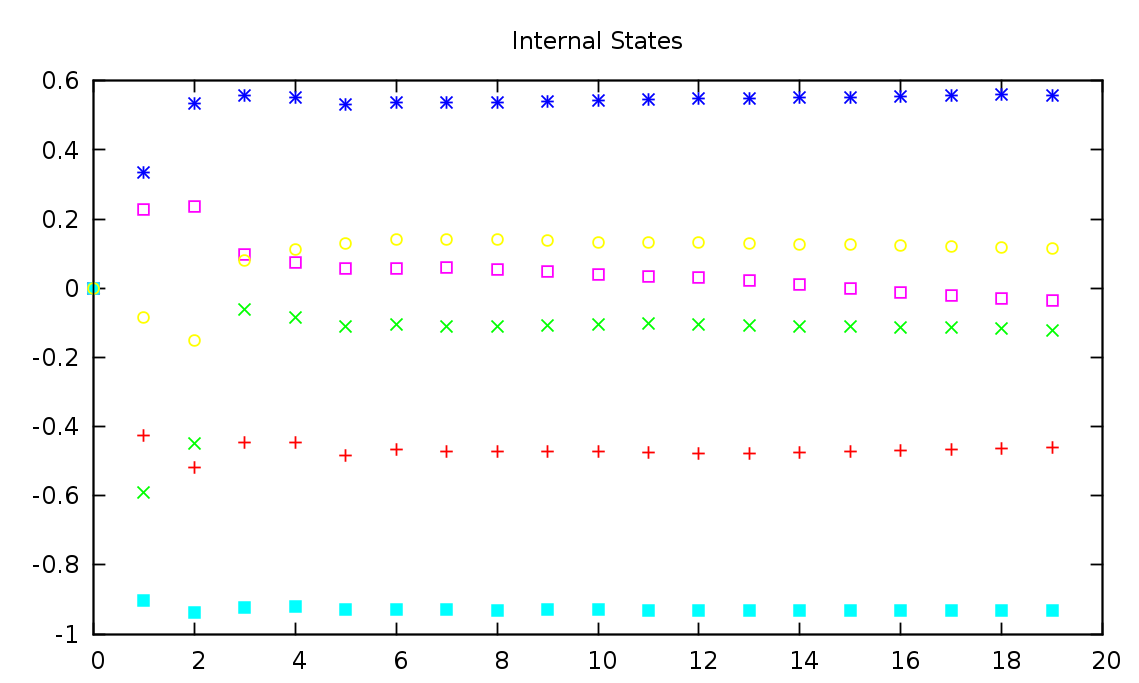
\includegraphics[height=120px]{Extra/walk_initial_states.png}
    \caption[Teacher Forced Internal States]{Value of the internal sates of a network driven by a signal.}
\end{figure}

It can be seen that the states quickly start oscillating smoothly. This indicates that the state of the network is evolving into a state suitable for training and that the behavior of the network is weakly influenced by the random initial state. For this research, fast networks with large leaking rates ($1/8$ being the smallest considered) were used. Networks with large leaking rates forget the internal state more quickly. Based on the plots and the leaking rates used, $20$ update cycles were discarded before training. This left enough data and enough transient for all experiments considered in this research. 

\subsection{Regularization Parameter Tuning}

The right complexity for the particular movement must be chosen. In this particular case it is rather unfeasible to observe the movements generated by different values of the regularization parameter $\lambda$. An automatic approach is suggested. Select two similar sequences of motion capture data. This can be two different walks for instance. A error measure can now be defined as follows. The network is trained with the movements of the first data set and the performance is tested by comparing the single step prediction of the network on the second data-set. Single step prediction is performed by running the network teacher forcing a signal and comparing the network output with the value of the signal. The following formulas illustrate the points:

\[
{\bf x}(t+1)={\bf f}({\bf Wx}(t)+{\bf W^{back}y_{test}}(t))
\]

\[
{\bf y}(t+1)={\bf f}({\bf W^{out}x}(t)+{\bf W^{back}y_{test}}(t))
\]

\[
MSE_{test} = \frac{1}{|test|}\sum_{t=0}^{|test|}\vectornorm{{\bf y_{test}}(t) - {\bf y} (t)}^2
\]

where,
\begin{itemize}
\item $\vectornorm{.}$ is the euclidean norm.
\item $|test|$ is the size of the testing set.
\end{itemize}

Many networks can be trained with different values for the regularization parameter and the chosen regularization parameter should be the one that minimizes the $E_{test}$ testing error.

\begin{figure}[h!]
  \centering
    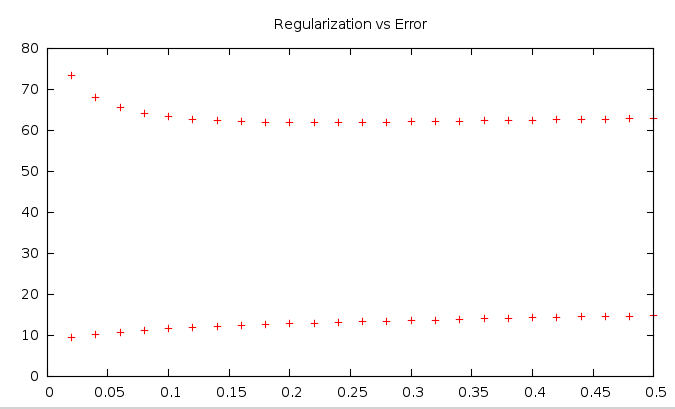
\includegraphics[height=150px]{Extra/regularization_vs_error.png}
    \caption[Error and Regularization]{The top line shows the error of a network with respect to the testing set and the bottom line shows the error of the network on the training set. It can be observed that the testing error starts decreasing as the regularization increases until it reaches the `right` complexity.}
\end{figure}

Choosing the regularization parameter this way usually was a good starting point, but never resulted in a good model for producing motions. This parameter is usually tuned by optimizing an error function for the network output. In this case this was manually done by looking at the generated movements since establishing an error assessment to evaluate how `good` the produced motion is goes beyond the scope of this research. An overfitted model usually results in `impossible` movements like an overfitted polynomial oscillating in ways that a polynomial of lower degree doesn't. On the other hand, too simplistic models usually result in convergence to fixed points or absence of detail in the movement.

\begin{figure}[h!]
  \centering
  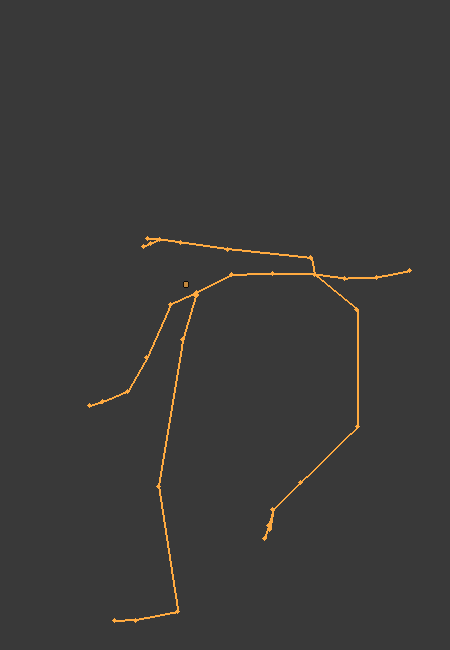
\includegraphics[height=150px]{Extra/overfitting_1.png}
  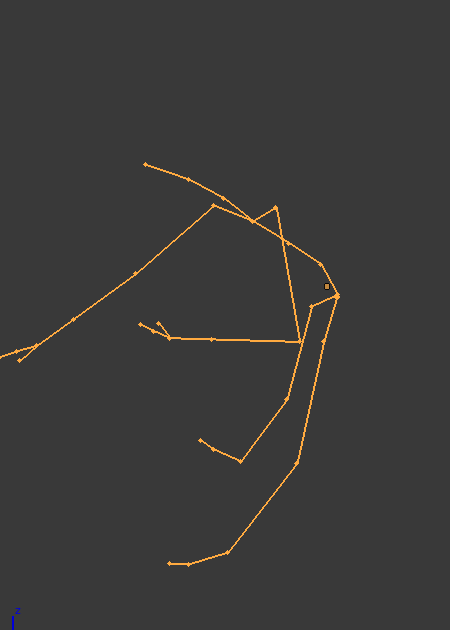
\includegraphics[height=150px]{Extra/overfitting_2.png}
  \caption[Error and Regularization]{This images show positions produced by an overfitted rowing motion. It is evident that the bending of the back and arms goes beyond what is present in the training set.}
\end{figure}


\subsection{Leaky Integrator Tuning}

The human movements considered during this research are continuous periodic signals. As it was previously mentioned, the leaky integrator is very important to simulate a continuous signal with a discrete network. The standard method to choose the leaking rate is minimizing an error function for output. In the case of human movements, minimizing the single step prediction error usually resulted in big leaking rates which produced chaotic motions. Therefore, to determine whether the leaky integrator is set to the right value the plots of the internal states during training and testing were observed. In the case of motion capture data, there should be smooth continuous oscillating patterns. No sudden jumps or chaotic behavior should be present. Once again this is not a black and white assessment, and as mentioned in \cite{ESNVerstraeten}, the network should be as chaotic as possible without falling into chaos.

\begin{figure}[h!]
  \centering
  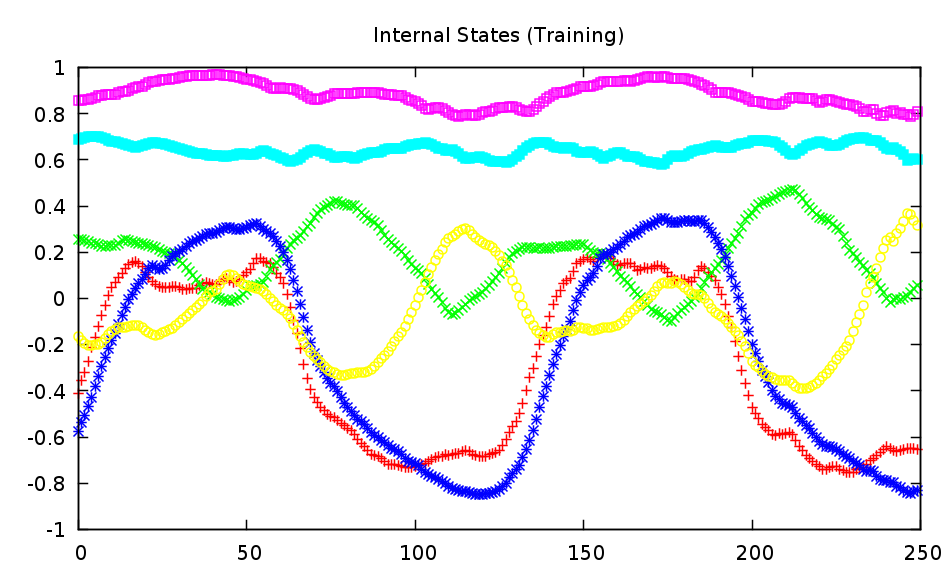
\includegraphics[height=125px]{Extra/sample_leaky_big.png}
  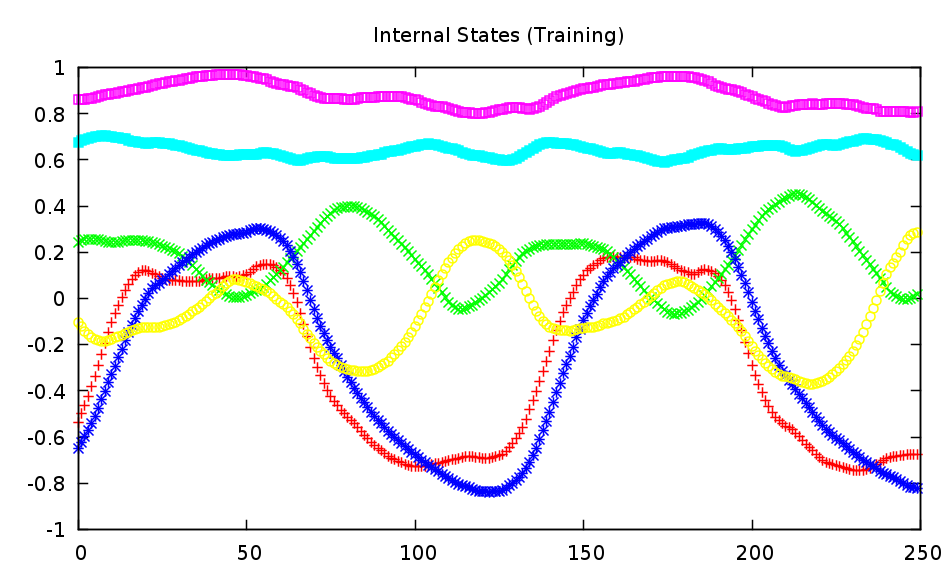
\includegraphics[height=125px]{Extra/sample_leaky_ok.png}
  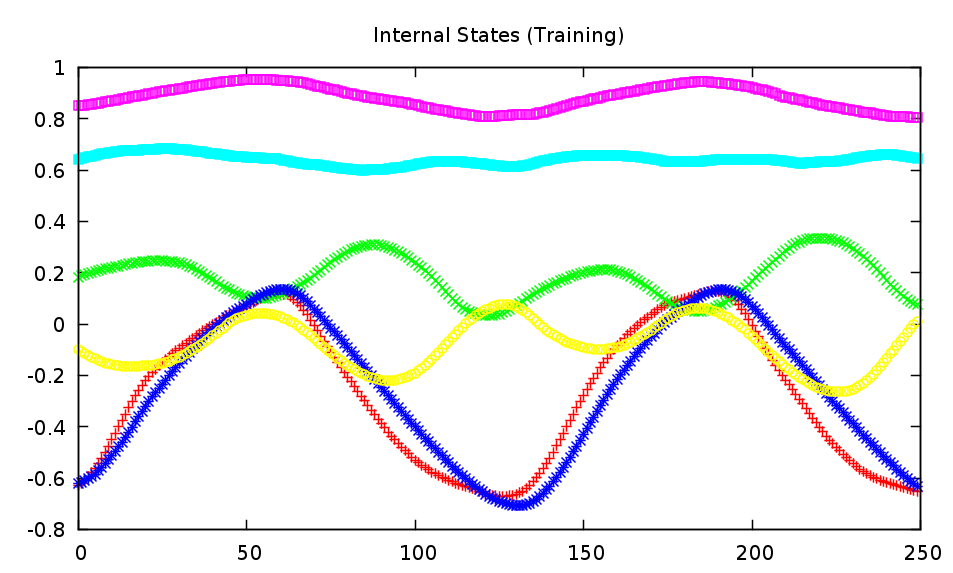
\includegraphics[height=125px]{Extra/sample_leaky_low.png}
    \caption[Leaky Integrator Comparison]{This figure shows the internal states of the same network with different value for the leaky integrator. The first network has a value close to one while the last has a value close to zero.}
\end{figure}

As it can be observed in the figure, when the leaking weight is too high, the network runs too fast and the states no longer evolve in a smooth and continuous matter. On the other hand, when the leaky integrator is to small, the network evolves so slow that the behavior of the internal states no longer captures the behavior of the teacher signal. It can be observed that the states oscillate less when the leaky integrator is too small. 

\subsection{Output Feedback Weights Tuning}

The dynamics of Echo State Networks used in this research heavily depend on the magnitude of the entries in the output feedback matrix ${\bf W^{back}}$. It is of crucial importance to tune these weights appropriately for the network to reproduce the input signal as realistically as possible. If the output feedback weights are to small, the network will not be excited enough to produce the signal. This results in a signal that behaves as if it were a more relaxed version of the original signal or the network might just converge to a fixed point. On the other hand, if the weights are too big, the network might behave chaotically or get squashed to border values.

\begin{figure}[h!]
  \centering
  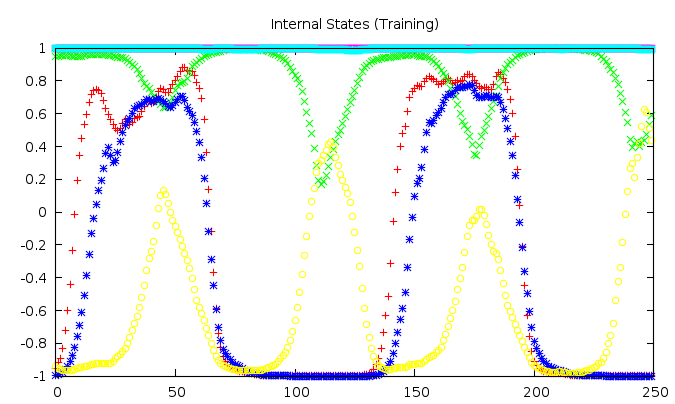
\includegraphics[height=125px]{Extra/ofbw_big.png}
  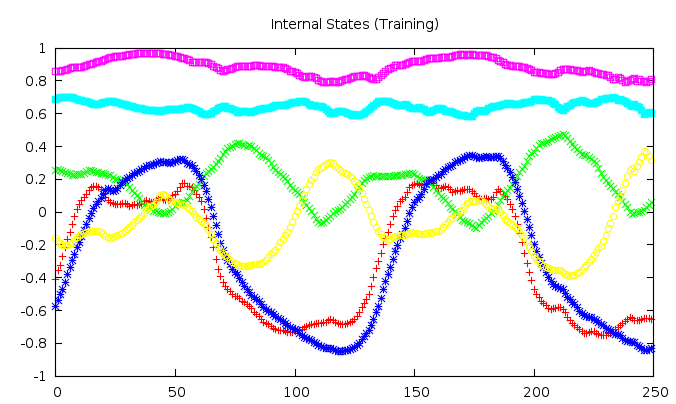
\includegraphics[height=125px]{Extra/ofbw_ok.png}
  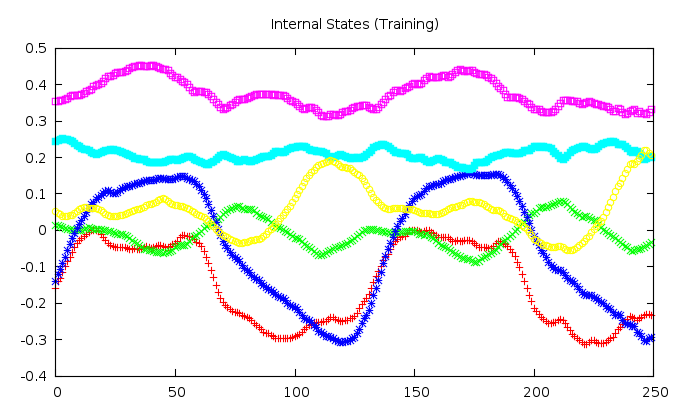
\includegraphics[height=125px]{Extra/ofbw_small.png}
    \caption[Output Feedback Weights Comparison]{This figure shows how big output feedback weights squash the value of the internal states close to -1 or 1 and how the small output feedback weights squash the values of the internal units into the non-linear region close to 0. The second plot shows a good selection of output feedback weights.}
\end{figure}

It is once again important to observe the internal states to determine whether the output feedback weights are of the right magnitude. To learn human movements, the hyperbolic tangent function $tanh$ was selected as the sigmond function for the internal units such that the function ${\bf f(x)}$ of equation 1 is defined as ${\bf f(x)} = (tanh(x_1),..,tanh(x_n))$. While observing the internal units of these networks it is important that the values of the internal units oscillate using the largest amount of values in the range $[-1,1]$ which is the range of the $tanh$ function. Large output feedback weights usually squash the values of the internal units either towards $-1$ or $1$. On the other hand, small output feedback weights usually squash the values towards a single value.

\begin{figure}[h!]
  \centering
  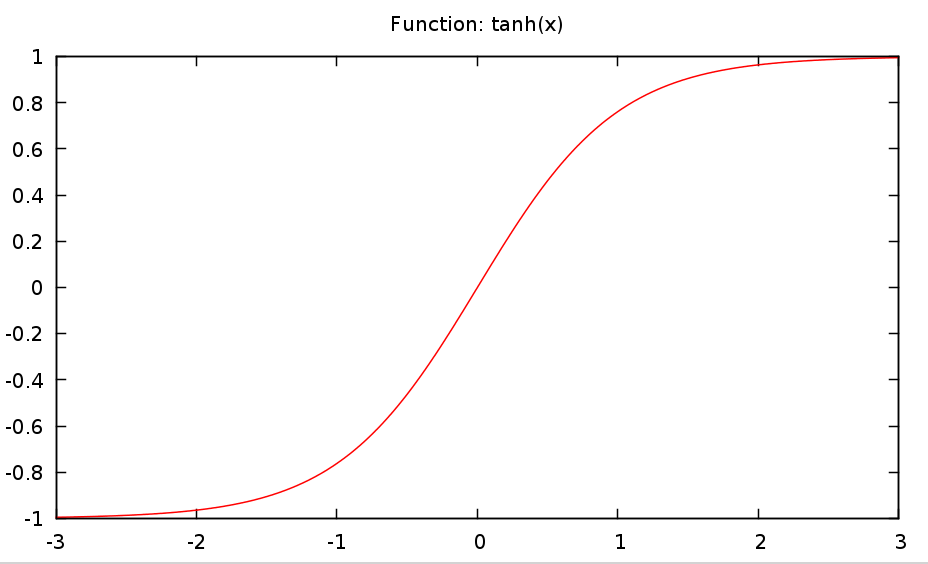
\includegraphics[height=125px]{Extra/tanh.png}
    \caption[Plot of $tanh(x)$ Function]{This figure shows a plot of the $tanh(x)$ function. It can be observed that the behavior of the function is almost linear for values close to zero.}
\end{figure}


The reasons why it is important to use as much values of the $tanh$ as possible are firstly the fact that the network is using a larger selection of values to learn a particular signal which gives the network more space to store information about the signal. The second reason is related to the behavior of the $tanh(x)$ function. As it can be seen in the picture, the $tanh(x)$ behaves like a linear function when values are close to 0 or when values become large or small. If the states stay squashed into one of these regions, the reservoir will behave like a linear dynamical system instead of behaving like a non-linear dynamical system.\\

It is important to begin tuning the network with reasonable magnitudes for the output feedback matrix. To outline what reasonable means, consider the update equation for the network. In this particular case $tanh(x)$ is being used as the network function. The entries of the current state ${\bf x(n)}$ are always between $[-1,1]$ and the entries of the internal weigh matrix ${\bf W}$ are usually small because of the scaling applied to the matrix in order to have a particular spectral radius. Therefore the value of each entry of the vector ${\bf Wx}(t)$ will also remain close to that range. This means that the other value ${\bf W^{back}y}(t)$ should oscillate around the range [-4,4] to ensure that the network remains nonlinear. It is important to inspect the teacher signal to bring these values into the range mentioned above. Often enough it is useful to globally scale the signal to choose these weights more easily (although global scaling is equivalent to scaling the ${\bf W^{back}}$ matrix).

%% \subsection{Spectral Radius Tuning}

%% As mentioned in \cite{JaegerESNTutorial}, the spectral radius $|\lambda |_{max}$ is very important to ensure the network has the echo state property and heavily influences the dynamics of the network. 

\subsection{Pre-Processing}

In many cases it is helpful or necessary to pre-process the teacher signal. In the case of motion capture data, the signal is already clean enough that no pre-processing is strictly necessary. However, to avoid having too small output feedback weights, the signal was globally scaled from the range $[0,180]$ to fit the range $[-0.5,0.5]$. The scaling was done by dividing all values in the teacher signal by the biggest value in the signal and subtracting $0.5$ from all entries.  

\subsection{Remarks}

It should be noted that before beginning the process of fine tuning the parameter, reasonable parameters for the leaking rate and feedback matrices should be chosen. The reason is that unreasonable values for these parameters can be spotted by inspecting the network behavior during training. As indicated previously, some negative indicators such as chaotic behavior or fixed points can be detected by inspecting the network states during training. Doing so is important because the way the network responds to the adjustment of a certain parameter depends on the values of the other parameters. Once a reasonable starting point is found, the network can be finely tuned by incrementally adjusting any of the parameters and inspecting the internal states and output of the network during training and testing.

\section{Results}

Different networks were built and trained to learn different movements. All of the movements are periodic motions and span different levels of complexity. Each of the movements emphasized motion of a particular set of bones and the network had to learn which were the important bones on each of the motions. The parameters used to build the network and results are provided. In the case of swimming and rowing, no similar data-set existed so to calculate the testing mean square error, an optimal network was produced using the full data-set and then the network was re-trained using the same parameters leaving out some data of the sequence for validation. Recall that the signal was rescaled to the range $[-0.5,0.5]$ when observing the mean squared error (MSE).

\subsection{Simple Walk}

This is the simplest motion of all. It consists of a periodic walk where only the movement of the legs is used as training data. An initial regularization parameter of $0.05$ was chosen using single step prediction against another walk but it was immediately evident that the model was over-fitted since the first walks produced movements which were not present in the training data. This is similar to over-fitting a polynomial with one of higher degree. The polynomial of higher degree will oscillate in ways that the other polynomial doesn't. The regularization parameter was experimentally lowered to $0.15$ by observing the generated output which finally produced a realistic and stable walk.

\begin{figure}[h!]
  \centering
  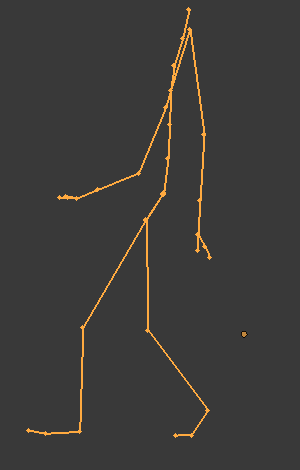
\includegraphics[width=100px]{Extra/out_simple_walk_1.png}
  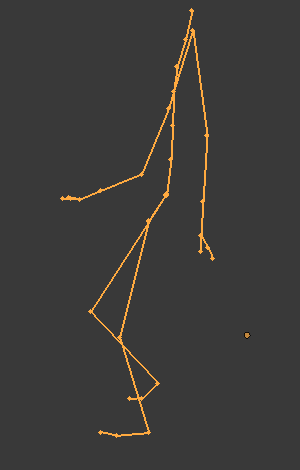
\includegraphics[width=100px]{Extra/out_simple_walk_2.png}
  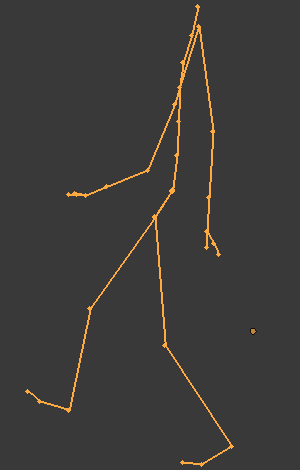
\includegraphics[width=100px]{Extra/out_simple_walk_3.png}\\
  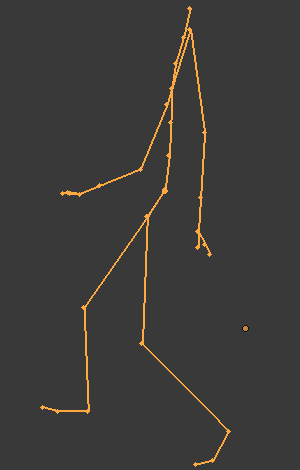
\includegraphics[width=100px]{Extra/teach_simple_walk_1.png}
  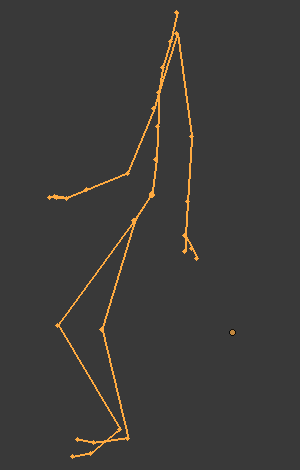
\includegraphics[width=100px]{Extra/teach_simple_walk_2.png}
  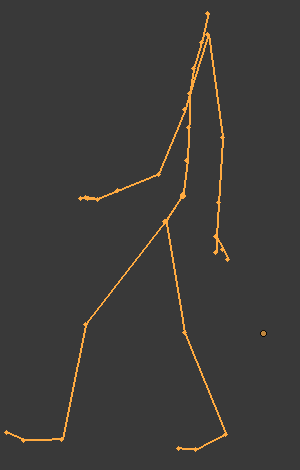
\includegraphics[width=100px]{Extra/teach_simple_walk_3.png}
    \caption[Simple Walk]{Comparison of the learned movement and the training movement. The thee images above are the motion produced by the network and the movements below are the motion used for training.}
\end{figure}

As it can be observed in the images the movement of legs looks very similar to the real movement. All the joints are folded as much as they should at the right moment of the sequence. Although that cannot be observed in pictures, the movements also occur at similar speed. The reader can visit \cite{LambdaNN} to see more videos of motions produced by the networks.

\subsection{Swimming}

\networkSpecs{0,0.1}
             {1.15}
             {-3/2,3/2}
             {1/5}
             {0.7}
             {25.77 over 239 steps}


Swimming involves the arms, legs and back which resulted in a much more complex motion. There were a total of $37$ degrees of freedom in the training data for the swimming motion. The training data was very short containing about four strokes which had some differences between each other. There was no other data-set available to use single step prediction to find the initial regularization parameter so $0.15$ was chosen based the results from the simple walk. This was too small and caused the produced output to converge into fixed points. When the regularization parameter is not big enough, the output weights result being too big. This creates an output that will easily squash the $tanh(x)$ into the corners resulting in convergence to a fixed point. This was the case for swimming even after selecting large and small output feedback weights. The regularizer was then gradually increased until 0.7 was found to produce realistic and stable strokes. Unfortunately the model produced after sparing some steps for the single step prediction was much worse than the original model. A complete stroke was used for validation and the resulting model looked overfitted.

\begin{figure}[h!]
  \centering
  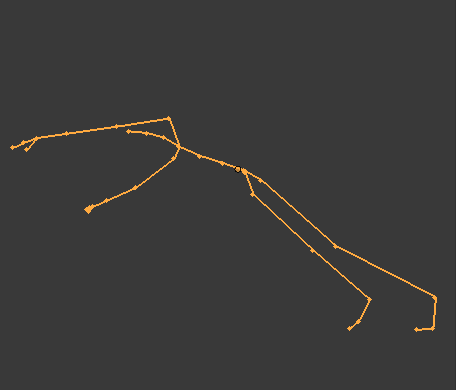
\includegraphics[width=100px]{Extra/out_swim_1.png}
  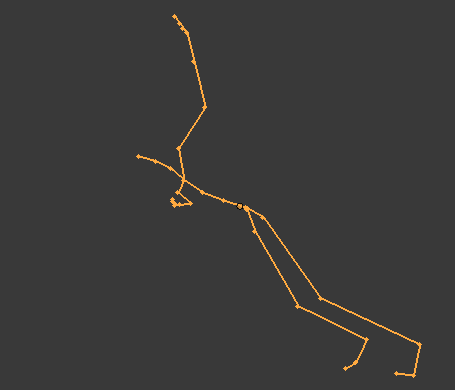
\includegraphics[width=100px]{Extra/out_swim_2.png}
  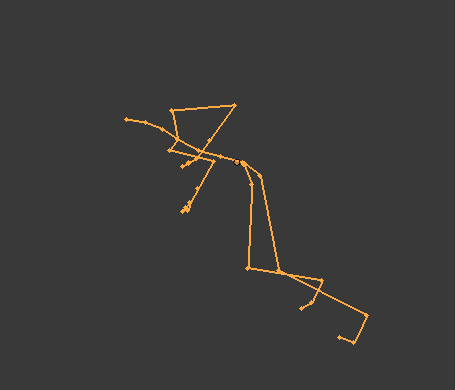
\includegraphics[width=100px]{Extra/out_swim_3.png}\\
  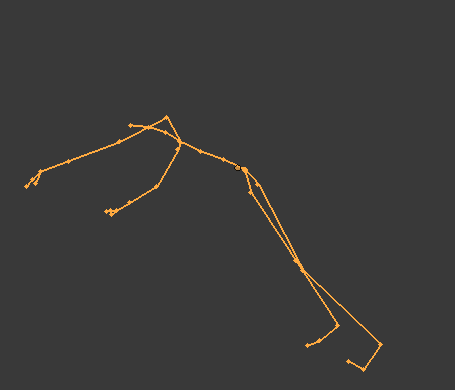
\includegraphics[width=100px]{Extra/teach_swim_1.png}
  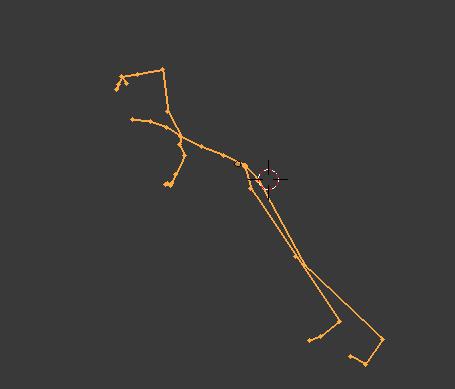
\includegraphics[width=100px]{Extra/teach_swim_2.png}
  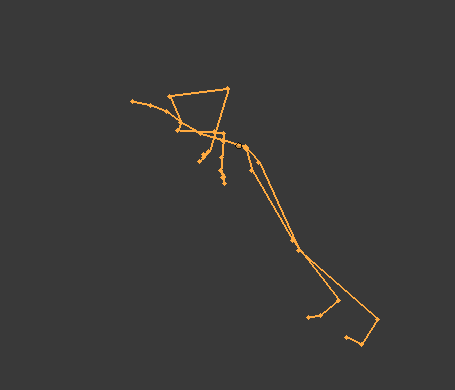
\includegraphics[width=100px]{Extra/teach_swim_3.png}
    \caption[Swimming]{Comparison of the learned movement and the training movement. The thee images above are the motion produced by the network and the movements below are the motion used for training.}
\end{figure}

It can be observed that the movements differ much more than in the case of the simple walk. The network generated stronger leg motion as it can be seen comparing the last image of the sequence. Nevertheless, it is difficult to compare by looking at the images, but the swimming motion generated by the network was similar to the training data. Both of them moved the arms and legs in similar cycles and both evolved at a similar pace. 

\subsection{Rowing}

\networkSpecs{0,0.1}
             {1.15}
             {-1,1}
             {1/6}
             {2}
             {15.21 over 80 steps}

Working with the rowing data was probably the most challenging task in this research. The data-set used was very small and the movement was complex since it involved $37$ degrees of freedom, all of which contained important motion. \\

According to the ``nature'' of Echo State Networks, rowing is a very different motion because the initial values in the range of $[0.15,0.3]$ for the regularization parameter produced an over-fitted model. The over-fitting was evident because even though the periodic nature of the motion was preserved and there were several poses which were similar in the training data and the produced motion, the generated motion contained bone rotations which are impossible for humans. This is analogous to an over-fitted polynomial which contains oscillations which are impossible in the polynomial of lower degree but still shares values in common with the lower degree polynomial. The network was finally trained by using a regularization value of $2$ which is considerably larger to the value used in the previous cases.\pagebreak

\begin{figure}[h!]
  \centering
  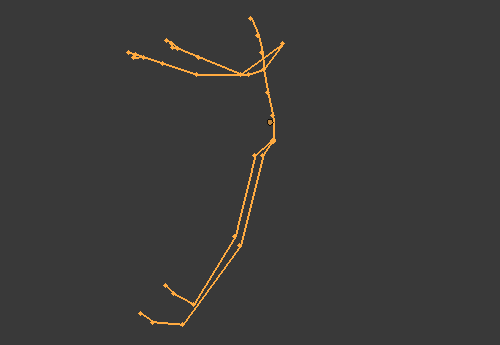
\includegraphics[width=100px]{Extra/out_row_1.png}
  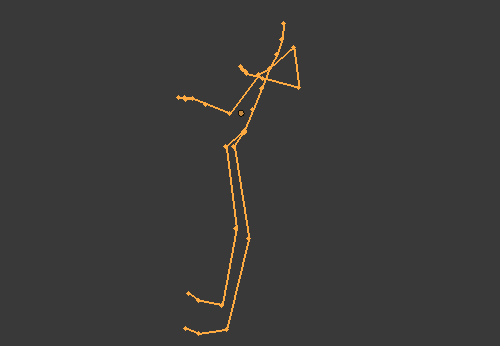
\includegraphics[width=100px]{Extra/out_row_2.png}
  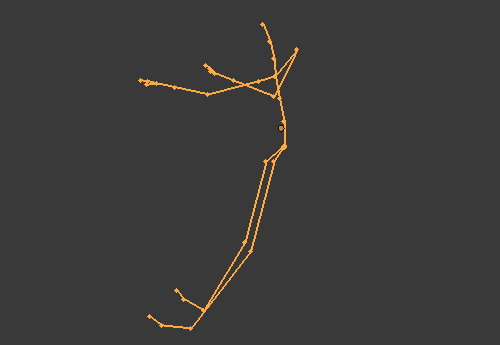
\includegraphics[width=100px]{Extra/out_row_3.png}\\
  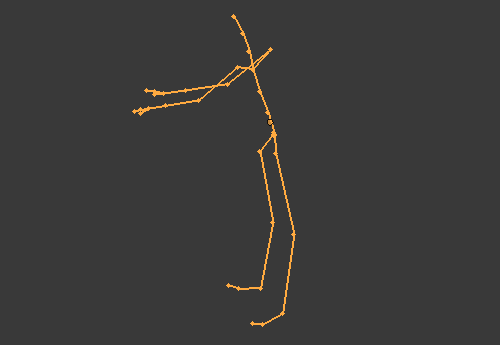
\includegraphics[width=100px]{Extra/teach_row_1.png}
  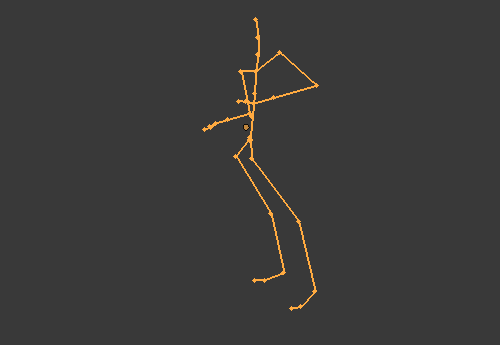
\includegraphics[width=100px]{Extra/teach_row_2.png}
  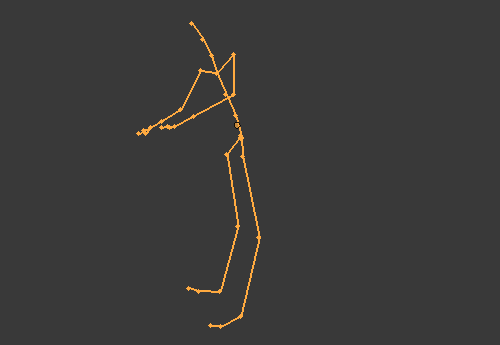
\includegraphics[width=100px]{Extra/teach_row_3.png}
    \caption[Rowing]{Comparison of the learned movement and the training movement. The thee images above are the motion produced by the network and the movements below are the motion used for training.}
\end{figure}

In the case of rowing, the network could correctly identify several of the poses adopted by the rower as well as the movements to go from one pose to the other. The biggest drawback in this case was speed and acceleration. The network seems to have a fixed speed and moves at that speed all the time. The speed at which a network evolves is controlled by the magnitude of the leaky integrator, but in this case the problematic part was the fact that the rowing motion is quicker during the stroke than during the return phase. The network couldn't correctly learn this feature and performs both segments at a similar speed.

\section{Discussion}

In spite of the small size of the training data-sets, the network successfully reproduced the movements that were taught. It is difficult to objectively asses the quality of the produced movements since the objective of this research was not to exactly imitate the movements but rather determine if the network was capable of correctly detecting the important features that the movements had such that it is capable of producing a realistic simulation of the motion without falling into chaos or convergence. Although the movements produced by the network were faithful to the original motion on many aspects. There were several drawbacks.\\

The first drawback encountered is over-emphasis of some of the positions. The network tended to bend some of the bones over a larger range of angular values than the training data. This can clearly be seen on figure 7 since the network bent the knees much more than the original motion. The method usually used to reduce the emphasis the network has over a movement is scaling the output feedback weights. The limitation in the case of swimming is that large output feedback weights were needed for the network to properly follow the movement of the arms since those movements were really strong and covered a big range of values. A compromise between the two movements had to be made to allow a good enough simulation of the original motion. \pagebreak

\begin{figure}[h!]
  \centering
  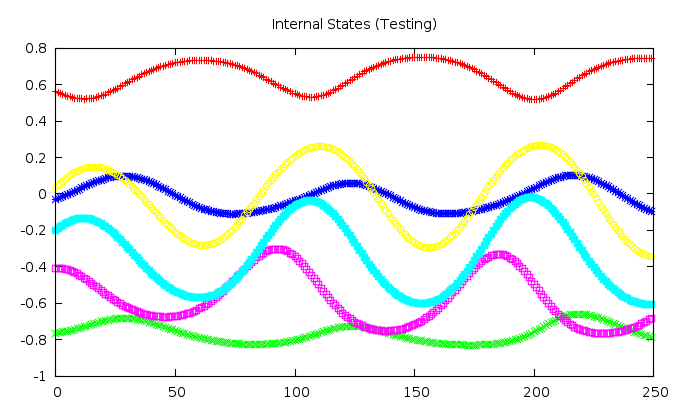
\includegraphics[width=200px]{Extra/out_states_rowing.png}
  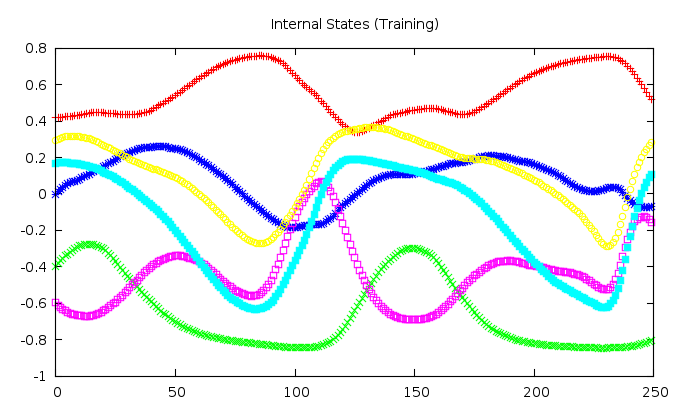
\includegraphics[width=200px]{Extra/train_states_rowing.png}
  \caption[Internal States Evolution]{The first image contains a plot of the internal states during the autonomous row and the second plot contains the states of the same network while being trained with rowing data. During the autonomous run, the network has a regular period whereas the training signal changes speed over time.}
\end{figure}

The second drawback is the difficulty the network had to learn to learn movements where the speed changes over time. Adjusting the intensity of the leaky integrator was useful to allow the network to learn motions of different paces such as walking and rowing but didn't prove useful to learn the speed variations of a movement. This had a negative impact in the rowing motion. A compromise for the leaky integrator had to be made such that the network was fast enough for the stroke and slow enough for the sliding section . It can clearly be seen in figure 10 that the value of the internal states changes at different speed over time during the training and during the autonomous run, the speed remains constant over time.\\

One of the main characteristics of ESNs is the fact that they are easy to create and train. This is because very few parameters have to be adjusted while tuning the network. In general this was the case for human movements. It was a matter of minutes to generate and tune the network for each of the movements learned in this work. This is also due to the low computational requirements of the networks since it was a matter of seconds to run the training algorithms on a regular computer. This was even so using an environment without fancy functionality such as the interactive Haskell shell.

\section{Future Work}

The first direction towards which the work presented here can be extended is by allowing motion which responds to input data as well. There exists work in a similar direction to use these networks to control robots in \cite{ESNRobots} such that the motion generated can adapt to the input from the sensors. With human motion it might get a little more difficult since there is no straightforward way to connect sensory input to motion capture data. A less provocative extension in this direction is running the network output in an environment that simulates physics. This way it can be researched how can the network be taught to move in a way that would not result in a catastrophe under more realistic conditions.\\

There is also a theoretical direction in which the work can be extended. It would be useful and interesting to produce networks that can learn the peculiarities of the different aspects of a single motion. This means having a network that suffers less from the shortcomings presented for rowing and swimming data. The reasoning behind having sparse matrices is allowing clusters with a particular behavior to be formed in the network to allow it to learn many of these peculiarities. A bigger network might allow more of these clusters to exist letting the network learn more aspects about the behavior of each of the components of the movement data signal. Understanding the memory limitations of the ESNs might also be helpful and such information is available in \cite{ESNMemory}.\\

The single step prediction method proposed in this work to choose the regularization parameter also has a lot of room for improvement. In the case of this research, the limited training data did not allow much room for performance assessments for the network. It was also difficult to judge the performance of the network since it was not trained to precisely reproduce a particular signal. Instead the objective of this work was to create motion that looked realistic so evaluation was mostly done by watching the generated movement on a skeleton. The network output could be automatically compared to another instance of the same movement but as mentioned in \cite{SimilarityMeasure}, comparing time series is a difficult task and is an active field of research. An automatic performance assessment would also allow more automated tuning since sub-optimal configurations such as over-fitting are currently detected and adjusted by manually inspecting the output.

\bibliographystyle{plain}
\bibliography{references}

\end{document}
